
\subsection{Implementierung}


\subsubsection{Code-Übersicht}
Das System besteht aus mehreren zentralen Komponenten:
\begin{itemize}
    \item \textbf{Datenbankverwaltung}: Die SQLite-Datenbank speichert Produktinformationen.
    \item \textbf{LLM-Interaktion}: Zwei LLMs werden verwendet:
    \begin{itemize}
        \item \textbf{Planer-LLM} (\texttt{llama3.1:latest}): Erstellt eine Handlungsstrategie basierend auf der Benutzeranfrage.
        \item \textbf{Executor-LLM} (\texttt{qwen2.5:14b}): F\"uhrt die geplanten Aktionen aus, insbesondere das Generieren und Ausf\"uhren von SQL-Statements.
    \end{itemize}
    \item \textbf{Speicherverwaltung}: \texttt{ConversationBufferMemory} speichert den Verlauf der Interaktion.
    \item \textbf{Agentenbasierte Steuerung}: Das System nutzt \texttt{PlanAndExecute}, um Anfragen zu beantworten.
\end{itemize}

\subsubsection{Datenbankverwaltung}
Die Datenbank \texttt{produkte.db} enth\"alt eine Tabelle \texttt{produkte} mit folgenden Spalten:
\begin{itemize}
    \item \texttt{product\_number} (Integer, Prim\"arschl\"ussel)
    \item \texttt{input\_voltage} (Integer)
    \item \texttt{input\_current} (Integer)
    \item \texttt{output\_voltage} (Integer)
    \item \texttt{output\_current} (Integer)
    \item \texttt{number\_io\_ports} (Integer)
    \item \texttt{bus\_protocol} (String)
\end{itemize}

\minisec{Verbindung zur Datenbank}
Die SQLAlchemy-Bibliothek wird zur Interaktion mit der SQLite-Datenbank verwendet:
\begin{lstlisting}[language=Python, style=pythonstyle, caption={Verbindung zur SQLite-Datenbank}]
DB_PATH = "./poc/db/produkte.db"
engine = create_engine(f"sqlite:///{DB_PATH}")
Session = sessionmaker(bind=engine)
database = SQLDatabase(engine)
\end{lstlisting}

\subsubsection{LLM-Interaktion}
\minisec{Initialisierung der Modelle}
\begin{lstlisting}[language=Python, style=pythonstyle, caption={Initialisierung der LLMs}]
planner_llm = ChatOllama(model="llama3.1:latest")
executor_llm = ChatOllama(model="qwen2.5:14b")
\end{lstlisting}

\minisec{Ged\"achtnisverwaltung}
\begin{lstlisting}[language=Python, style=pythonstyle, caption={Speicherung der Konversationshistorie}]
memory = ConversationBufferMemory(memory_key="chat_history", return_messages=True)
\end{lstlisting}

\minisec{Werkzeuge f\"ur SQL-Interaktion}
\begin{lstlisting}[language=Python, style=pythonstyle, caption={Definition der SQL-Tools}]
tools = [
    Tool(
        name="SelectQuery",
        func=select_query,
        description="Führt SQL-SELECT-Abfragen aus."
    ),
    Tool(
        name="ExecuteUpdateQuery",
        func=execute_update_query,
        description="Führt SQL-UPDATE-Statements aus."
    )
]
\end{lstlisting}

\subsubsection{Plan-and-Execute Agent}
Der Agent verarbeitet Benutzeranfragen mit folgendem Workflow:
\begin{enumerate}
    \item \textbf{Planung}: Das \texttt{planner\_llm} analysiert die Anfrage und erstellt eine Aufgabenliste.
    \item \textbf{Ausf\"uhrung}: Das \texttt{executor\_llm} f\"uhrt die geplanten Aktionen aus.
    \item \textbf{R\"uckgabe der Antwort}: Das Ergebnis wird an den Benutzer zur\"uckgegeben.
\end{enumerate}

\begin{lstlisting}[language=Python, style=pythonstyle, caption={Definition des Agents}]
planner = load_chat_planner(planner_llm)
executor = load_agent_executor(executor_llm, tools, verbose=True)
agent = PlanAndExecute(planner=planner, executor=executor, verbose=True)
\end{lstlisting}




\subsection{Prozess}

\begin{figure}[H]
    \centering
    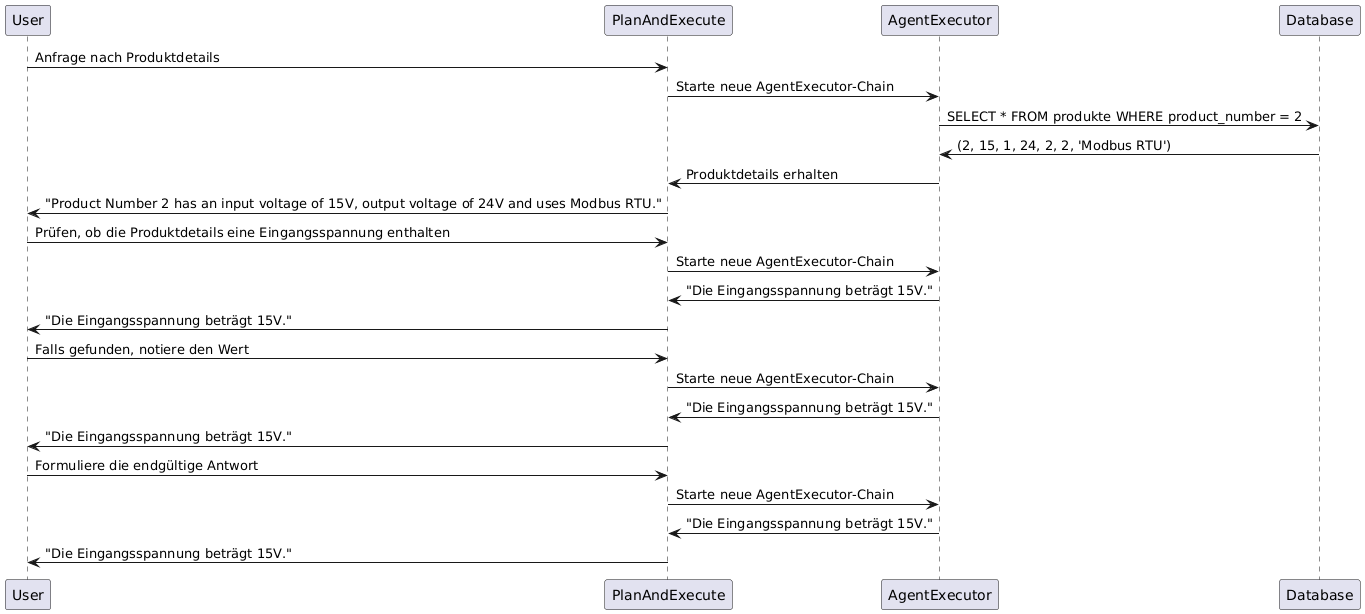
\includegraphics[width=1\textwidth]{Figures/diagramms/activity-chain.png}
    \caption{Multi-Modell-Architektur ABlauf der Chain}
    \label{fig:multi-model-architecture}
\end{figure}

Die Kette wird mehrfach ausgeführt, da der PlanAndExecute-Agent die Aufgabe in mehrere Schritte unterteilt und für jeden einzelnen Schritt eine neue AgentExecutor-Kette startet. Der Prozess ist wie folgt (Genauer Ablauf unter \autoref{lst:chain-content}):

\textbf{Planung:}
\begin{itemize}
    \item Die PlanAndExecute-Kette erstellt eine Liste von Schritten, um die Frage zu beantworten.
    \item In diesem Fall ist die Abfolge der Schritte wie folgt:
    \begin{itemize}
        \item Abrufen der Produktdetails für Produktnummer 2 aus einer Datenbank.
        \item Überprüfen, ob die Produktdetails Informationen zur Eingangsspannung enthalten.
        \item Falls verfügbar, die Eingangsspannung notieren.
        \item Formulieren der endgültigen Antwort basierend auf den obigen Schritten.
    \end{itemize}
\end{itemize}

\textbf{Ausführung:}
\begin{itemize}
    \item Für jeden dieser Schritte wird eine separate AgentExecutor-Kette gestartet.
    \item Dies führt dazu, dass die Datenbankabfrage indirekt mehrfach verarbeitet wird, selbst wenn die Informationen bereits bekannt sind.
\end{itemize}

\textbf{Grund für dieses Verhalten:}
\begin{itemize}
    \item PlanAndExecute ist so konzipiert, dass jeder Schritt unabhängig behandelt und mit einem AgentExecutor implementiert wird.
    \item Es scheint, dass dem Agenten ein Mechanismus fehlt, um zu erkennen, dass alle relevanten Daten bereits gesammelt wurden, bevor er zum nächsten Schritt übergeht.
    \item Dies führt zu redundanten Aktionen (mehrere AgentExecutor-Instanzen für ähnliche Informationen).
\end{itemize}

\textbf{Mögliche Lösungen:}
\begin{itemize}
    \item \textbf{Speicher optimieren:}
    \begin{itemize}
        \item Sicherstellen, dass ConversationBufferMemory korrekt verwendet wird und vorherige Antworten speichert.
        \item Überprüfen, ob der Agent tatsächlich auf vorherige Schritte zugreift oder sie jedes Mal neu berechnet.
    \end{itemize}
    \item \textbf{Benutzerdefinierte Logik für PlanAndExecute:}
    \begin{itemize}
        \item Wenn möglich, die PlanAndExecute-Logik so anpassen, dass sie nicht automatisch jeden Schritt ausführt, sondern überprüft, ob die Daten bereits verfügbar sind.
    \end{itemize}
    \item \textbf{Debugging:}
    \begin{itemize}
        \item Logging verwenden, um zu überprüfen, welche Zwischenergebnisse tatsächlich an den nächsten Schritt übergeben werden.
    \end{itemize}
\end{itemize}